\section{Interactivité}
\label{s:interactivité}

Il y a deux modes d'interaction avec l'application: le clavier et la souris.
Le clavier est utilisé pour entrer des raccourcis permettant d'effectuer des actions alors que la souris permet de contrôler les éléments de l'interface graphique.

\subsection{Raccourcis clavier}
Les raccourcis clavier disponible sont les suivants:

\begin{table}[h]
    \begin{center}
    \begin{tabular}{|c|l|}
        \hline
        \multicolumn{1}{|c|}{Touche} & \multicolumn{1}{c|}{Action}\\
        \hline
        CTRL + Z & \emph{Undo}\\
        CTRL + Y & \emph{Redo}\\
        Espace & Capture d'écran\\  
        Flèches gauche/droite & Rotation de la caméra autour de son axe Y local\\
        Flèches haut/bas & Rotation de la caméra autour de son axe X local\\
        A/D & Déplacement de la caméra sur son axe X local\\
        W/S & Déplacement de la caméra sur son axe Y local\\
        +/- & Déplacement de la caméra sur son axe Z local\\
        H & Afficher/cacher l'interface graphique\\
        1 & Créer une sphère\\
        2 & Créer un cube\\
        3 & Créer une ligne\\
        4 & Créer un triangle\\
        5 & Créer un rectangle\\
        6 & Créer un pentagone\\
        7 & Créer un cercle\\
        8 & Créer une flèche\\
        9 & Créer une étoile\\
        M & Créer un modèle 3D du Faucon Millenium\\
        X & Créer un modèle 3D d'un X-Wing Fighter\\
        \hline
    \end{tabular}
    \caption{Raccourcis claviers de l'application}
    \end{center}
\end{table}
Il est à noter que les touches \emph{CTRL} droite et gauche fonctionnent pour les actions \emph{Undo} et \emph{Redo}.
De plus, le contrôle de la caméra s'effectue toujours dans son repère local.\\

\subsection{Interface graphique}
L'interface graphique comporte trois panneaux.
Le premier est appelé \emph{Inspecteur} et se situe à droite de l'écran (voir figure \ref{fig:inspecteur}).
Il permet de modifier les attributs de l'objet présentement sélectionné et apparait après avoir créer un premier objet.
L'inspecteur permet de modifier la position, la rotation, l'échelle, la couleur ainsi que le parent d'un objet dans le graphe de scène.\\

La position est modifiée à l'aide de trois champs de textes permettant d'entrer des valeurs numériques entre -1000 et 1000 pour les composantes x, y et z.
Si l'utilisateur entre une valeur à l'extérieur de cette intervalle, celle-ci est ramenée à la limite la plus proche.
S'il entre un caractère non numérique (sauf le signe moins), alors le champ est remis à 0.
La rotation d'objet est modifiée à l'aide de trois glisseurs permettant de sélectionner une valeur entre -180 et 180 degrés pour chacun des angles d'Euler.
L'échelle est modifiée à l'aide de trois champs de textes similaires à ceux pour la position, mais limités entre -100 et 100. Les valeurs de position, de rotation et d'échelle affichées dans l'inspecteur sont dans le référentiel local de l'objet sélectionné, ce qui veut dire que s'il est enfant d'un autre objet, les valeurs affichées seront par rapport au parent et non par rapport au référentiel global de la scène.\\


\begin{figure}[H]
    \centering
	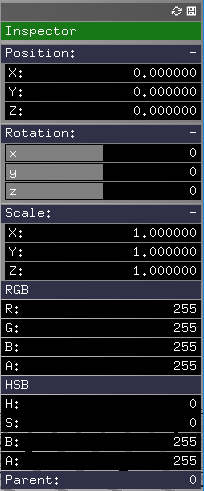
\includegraphics[scale=0.6]{fig/inspecteur.png}
	\caption{Inspecteur}
	\label{fig:inspecteur}
\end{figure}

En dessous de ces contrôles se trouvent deux groupes de quatre champs de nombres entiers permettant de modifier la couleur de l'objet sélectionné.
Les quatre premiers représentent les composantes \emph{rgba} de la couleur de l'objet, alors que les quatre autres représentent les composantes \emph{hsba} de la même couleur. Chacun des champs est limité à l'intervalle de 0 à 255. Modifier une valeur dans un groupe de quatre champs modifient les valeurs dans l'autre groupe de façon simultanée.\\

Le dernier contrôle présent dans l'inspecteur est un champ de nombre entier permettant de sélectionner le parent de l'objet sélectionné dans le graphe de scène.
Cette valeur doit être comprise entre 0 et le nombre d'objets dans la scène inclusivement, 0 signifiant que l'objet n'a pas de parent.
Un nombre supérieur à 0 représente le numéro de l'objet parent dans la liste des objets de la scène, 1 étant le premier, 2 le deuxième et ainsi de suite.
Un objet ne peut pas être son propre parent ni être l'enfant d'un de ses enfants.\\

Le second panneau est appelé \emph{Scène} et il se situe en haut à gauche de l'écran (voir figure \ref{fig:scene}).
Il affiche la liste des objets présents dans la scène.
Il est possible de sélectionner un objet en cliquant sur le petit bouton à gauche de son nom dans la liste, ce qui modifie les valeurs affichées dans l'inspecteur à celles du nouvel objet sélectionné.
Les objets sont affichés dans la liste dans l'ordre qu'ils sont créés et leur ordre n'est pas modifiable.
Le numéro d'un objet de la scène correspond à son ordre dans la liste, débutant à 1.\\

\begin{figure}[H]
    \centering
	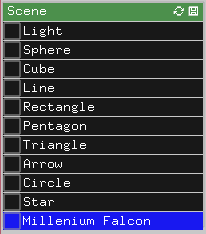
\includegraphics[scale=0.6]{fig/scene.png}
	\caption{Scène}
	\label{fig:scene}
\end{figure}

Le dernier panneau de contrôle est celui des textures (voir figure \ref{fig:texture}).
Il s'affiche en bas à gauche de l'écran uniquement lorsqu'un objet 2D (ligne, rectangle, triangle, cercle ou pentagone) est sélectionné.
Ce panneau permet de choisir la texture de l'objet 2D parmi les 5 textures procédurales offertes.

\begin{figure}[H]
    \centering
	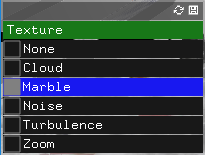
\includegraphics[scale=0.6]{fig/texture.png}
	\caption{Texture}
	\label{fig:texture}
\end{figure}
